% Apresentação intermediária da PoC OCR-06 (INE5448, 13/10/2026)
\documentclass[aspectratio=169,11pt]{beamer}
\usetheme{metropolis}
\usepackage[utf8]{inputenc}
\usepackage[T1]{fontenc}
\usepackage[brazil]{babel}
\usepackage{booktabs}
\usepackage{tikz}
\usetikzlibrary{positioning,arrows.meta,fit,backgrounds}
\metroset{progressbar=frametitle, numbering=fraction}
\setbeamertemplate{caption}{\insertcaption}

\title{OCR-06: OCR Adaptativo com Aprendizagem Assistida}
\subtitle{Apresentação intermediária da PoC}
\author{Gabriel Salmoria \quad {\small Tutor: Lucas Mayr}}
\institute{INE5448 -- IA e Segurança -- UFSC}
\date{13 de outubro de 2026}

\begin{document}

\maketitle

% ------------------------------------------------------------------ problema
\begin{frame}{Problema e objetivo}
\textbf{Problema}
\begin{itemize}
  \item OCRs com VLM leem bem texto comum, mas trocam nomes raros por palavras mais prováveis
  \item Num cartório, um nome com uma letra errada já invalida o registro
  \item O operador corrige à mão e o modelo continua errando o mesmo nome
\end{itemize}
\vspace{0.6em}
\textbf{Objetivo}
\begin{itemize}
  \item Reduzir o CER em nomes próprios manuscritos, principalmente nos que o modelo nunca viu
  \item Sem piorar a leitura do texto geral
  \item Sem o modelo decorar dados de pessoas reais
\end{itemize}
\end{frame}

% ------------------------------------------------------------------ solução
\begin{frame}{Solução proposta}
\begin{itemize}
  \item \emph{Fine-tuning} com LoRA do \textbf{Chandra OCR 2}, modelo aberto de OCR derivado do Qwen3.5-4B
  \item Treino com dois tipos de linha manuscrita:
  \begin{itemize}
    \item \textbf{BRESSAY}: 1.000 redações reais com transcrição (caligrafia real)
    \item \textbf{Sintéticas}: nomes, sobrenomes e municípios de dados públicos (IBGE, TSE, Receita), desenhados com fontes manuscritas e degradados com Augraphy
  \end{itemize}
  \item Treino majoritariamente sintético: nomes reais da população combinados aleatoriamente, então nenhuma linha corresponde a uma pessoa
  \item Memória de correções (RAG com FAISS): mantida como complemento, só se sobrar tempo
\end{itemize}
\end{frame}

% ------------------------------------------------------------------ arquitetura
\begin{frame}{Arquitetura}
\centering
\resizebox{!}{0.8\textheight}{%
\begin{tikzpicture}[
    font=\scriptsize,
    box/.style={draw, rounded corners=2pt, align=center, minimum height=0.85cm, text width=2.3cm, fill=white},
    plan/.style={box, dashed},
    arr/.style={-{Stealth[length=2mm]}},
    lane/.style={draw=gray!50, rounded corners=4pt, inner sep=5pt}]
  \node[box] (fontes) {IBGE, TSE,\\Receita Federal};
  \node[box, right=0.45cm of fontes] (lexico) {Léxico agregado\\(contagens)};
  \node[box, right=0.45cm of lexico] (vocab) {Vocabulário por\\frequência};
  \node[box, right=0.45cm of vocab] (gerador) {Renderização +\\Augraphy};
  \node[box, below=0.35cm of fontes] (bressay) {BRESSAY\\(Zenodo)};
  \node[box, right=0.45cm of bressay] (limpeza) {Limpeza +\\marcação de nomes};
  \node[box, below=0.35cm of gerador] (mistura) {Mistura\\train / val / test};
  \draw[arr] (fontes) -- (lexico);
  \draw[arr] (lexico) -- (vocab);
  \draw[arr] (vocab) -- (gerador);
  \draw[arr] (gerador) -- (mistura);
  \draw[arr] (bressay) -- (limpeza);
  \draw[arr] (limpeza) -- (mistura);
  \begin{scope}[on background layer]
    \node[lane, fit=(fontes)(gerador)(bressay)(mistura), label={[font=\scriptsize\bfseries]above left:Dados (CPU), pronto}] {};
  \end{scope}
  \node[box, below=1.0cm of bressay] (chandra) {Chandra OCR 2\\(BF16)};
  \node[box, right=0.45cm of chandra] (lora) {LoRA\\(transformers + peft)};
  \node[box, right=0.45cm of lora] (fp8) {Fusão + FP8\\(llm-compressor)};
  \node[box, right=0.45cm of fp8] (vllm) {Inferência\\(vLLM)};
  \node[box, below=0.35cm of vllm] (aval) {Avaliação\\CER / WER};
  \node[plan, below=0.35cm of fp8] (rag) {Memória RAG\\(planejada)};
  \node[box, below=0.35cm of chandra] (base) {Baseline:\\Chandra FP8};
  \draw[arr] (chandra) -- (lora);
  \draw[arr] (lora) -- (fp8);
  \draw[arr] (fp8) -- (vllm);
  \draw[arr] (vllm) -- (aval);
  \draw[arr, dashed] (rag) -- (vllm);
  \node[below=0.25cm of base, inner sep=0pt, minimum size=0pt] (bot) {};
  \draw[arr] (base.south) -- (bot.center) -| (aval.south);
  \draw[arr] (mistura.south) -- ++(0,-0.45) -| (lora.north);
  \draw[arr] (mistura.south) -- ++(0,-0.45) -| (vllm.north);
  \begin{scope}[on background layer]
    \node[lane, fit=(chandra)(vllm)(aval)(base)(rag)(bot), label={[font=\scriptsize\bfseries]below left:Modelo (GPU, servidor), scripts prontos}] {};
  \end{scope}
\end{tikzpicture}}
\end{frame}

% ------------------------------------------------------------------ fluxo
\begin{frame}[fragile]{Fluxo}
\small
Tudo roda por dois scripts, igual no notebook e no servidor:
\begin{verbatim}
scripts/setup.sh     # 3 ambientes: dados, treino, vLLM (detecta a GPU)
scripts/run.sh       # tudo, ou etapas avulsas:
\end{verbatim}
\vspace{-0.6em}
\begin{columns}[T]
\begin{column}{0.48\textwidth}
\textbf{Dados (CPU)}
\begin{enumerate}
  \item \texttt{lexicon}: coleta e agrega nomes
  \item \texttt{fonts}: fontes manuscritas
  \item \texttt{bressay}: download, limpeza, nomes
  \item \texttt{generate}: imagens sintéticas
  \item \texttt{mix}: conjuntos finais
  \item \texttt{exp1}: Experimento 1
\end{enumerate}
\end{column}
\begin{column}{0.48\textwidth}
\textbf{Modelo (GPU)}
\begin{enumerate}
  \item \texttt{baseline}: Chandra sem treino
  \item \texttt{treino}: LoRA com parada antecipada
  \item \texttt{quantizar}: fusão + FP8
  \item \texttt{avaliacao}: CER/WER e tabela final
\end{enumerate}
\end{column}
\end{columns}
\end{frame}

% ------------------------------------------------------------------ desenvolvido
\begin{frame}{O que já foi desenvolvido: dados}
\begin{columns}[T]
\begin{column}{0.5\textwidth}
\textbf{Nomes (dados públicos)}
\begin{itemize}
  \item 100.511 prenomes do Censo 2010 (IBGE)
  \item 60.627 sobrenomes contados em 4,07 milhões de candidatos (TSE) e sócios (Receita)
  \item 5.570 municípios com população do Censo 2022
  \item Nomes completos nunca vão pro disco: só contagens por palavra
\end{itemize}
\end{column}
\begin{column}{0.5\textwidth}
\textbf{Conjuntos finais}
\begin{itemize}
  \item Treino: 56.915 linhas (40.000 sintéticas + 16.915 do BRESSAY, 29,7\% reais)
  \item Validação: 6.074 linhas
  \item Teste sintético: 4.000 linhas, 8.629 nomes nunca vistos no treino
  \item Teste BRESSAY: 5.146 linhas de autores fora do treino
\end{itemize}
\end{column}
\end{columns}
\end{frame}

% ------------------------------------------------------------------ demo
\begin{frame}{Demonstração: linhas sintéticas}
\centering
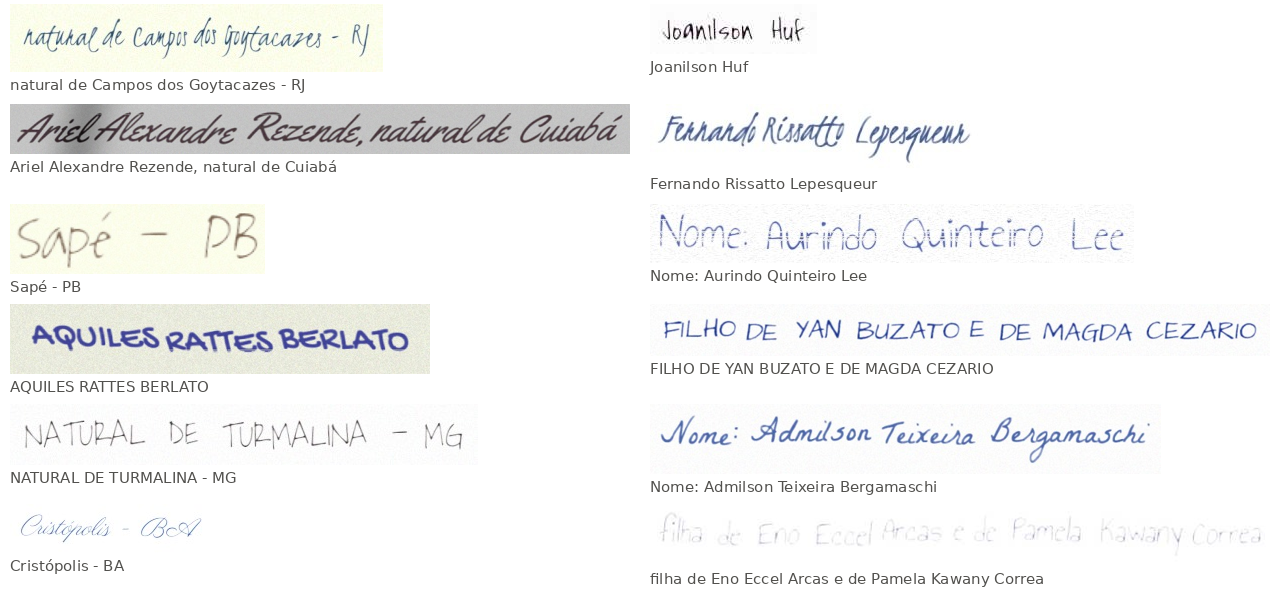
\includegraphics[height=0.72\textheight]{figs/exemplos_sinteticos.png}

\small 46 mil imagens geradas em 12,5 min (16 núcleos, sem GPU), 873 MB
\end{frame}

% ------------------------------------------------------------------ decisões
\begin{frame}{Decisões técnicas: quais nomes entram}
\small
\begin{itemize}
  \item Nomes entram por \textbf{frequência real} até cada um aparecer pelo menos 2 vezes no treino. Com 40 mil imagens: 10 mil prenomes (94\% da população), 19 mil sobrenomes, 3,8 mil municípios
  \item Temperatura $q_i \propto p_i^{0{,}5}$: o top-10 de prenomes cai de 21\% para 2,3\% dos sorteios. 10\% dos nomes raros ficam só no teste
\end{itemize}
\centering
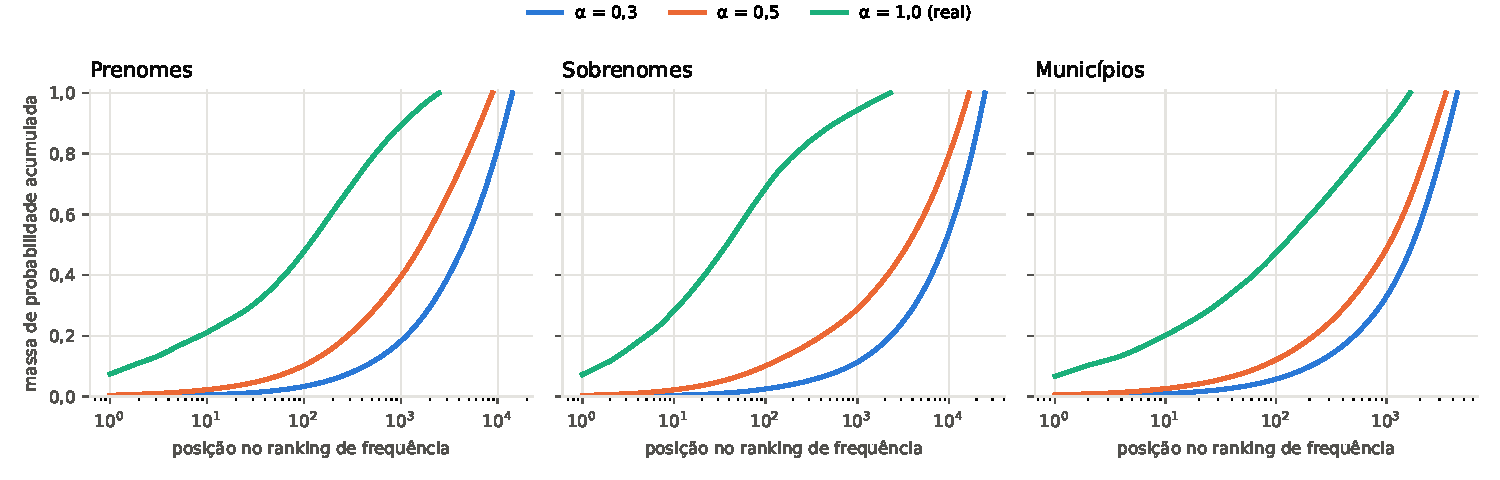
\includegraphics[height=0.47\textheight]{figs/massa_acumulada.pdf}
\end{frame}

\begin{frame}{Decisões técnicas: modelo e infraestrutura}
\begin{itemize}
  \item \textbf{Chandra OCR 2} em vez de VLM genérico: já faz OCR de manuscrito, e a config é idêntica à do Qwen3.5-4B
  \item \textbf{Treino em BF16, inferência em FP8}: FP8 no \texttt{transformers} é só inferência; a L40S (48 GB) cabe o modelo inteiro
  \item \textbf{FP8 próprio depois do treino}, com a mesma receita do FP8 público do Chandra, pra comparação justa
  \item \textbf{\texttt{transformers} + \texttt{peft}} em vez de Unsloth: sem suporte confirmado para Qwen3.5
  \item \textbf{3 ambientes Python}: vLLM e treino exigem versões diferentes de torch/transformers
\end{itemize}
\end{frame}

% ------------------------------------------------------------------ segurança
\begin{frame}{Segurança e privacidade}
\begin{columns}[T]
\begin{column}{0.5\textwidth}
\textbf{Já implementado}
\begin{itemize}
  \item TSE/Receita: só contagens; zips apagados; sobrenomes com $< 5$ ocorrências descartados
  \item Treino com no máximo 45\% de dado real (o script falha acima disso)
  \item Partição do BRESSAY por autor e nomes reservados ao teste
  \item Geração determinística e MD5 do BRESSAY conferido
\end{itemize}
\end{column}
\begin{column}{0.5\textwidth}
\textbf{Previsto}
\begin{itemize}
  \item Memorização: CER em nomes vistos vs.\ inéditos e tentativa de extração
  \item Injeção de instruções pela imagem: saída restrita a transcrição e revisão humana nas linhas de baixa confiança
  \item Confiança por palavra (log-probabilidades do vLLM) para o operador
\end{itemize}
\end{column}
\end{columns}
\end{frame}

% ------------------------------------------------------------------ dificuldades
\begin{frame}{Dificuldades encontradas}
\begin{itemize}
  \item \textbf{Sem acesso ao servidor com GPU até agora}: nenhum baseline ou treino rodou. A parte de dados foi antecipada e a de modelo ficou pronta em código, pra rodar com dois comandos
  \item \textbf{Nomes do BRESSAY são autores citados} (Bauman, Freud, Machado de Assis): dos 548 nomes no teste real, só 38 são inéditos. A métrica de nomes inéditos depende do teste sintético
  \item \textbf{Unsloth sem suporte confirmado para Qwen3.5}: troca por \texttt{transformers} + \texttt{peft}
  \item \textbf{Resolução das linhas reais} (próximo slide)
\end{itemize}
\end{frame}

\begin{frame}{Dificuldade: resolução do BRESSAY}
\centering
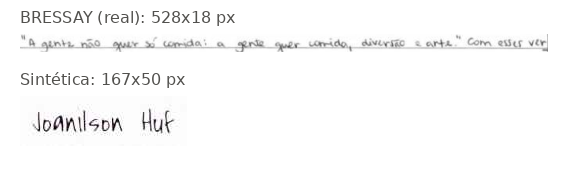
\includegraphics[height=0.42\textheight]{figs/resolucao.png}
\small
\begin{itemize}
  \item BRESSAY: altura mediana de 20 px (5\% a 95\% entre 15 e 38 px). Sintéticas: 48 a 112 px
  \item O Chandra divide a imagem em blocos de 32 px: a linha real vira menos de um bloco de altura
  \item Ajuste previsto: redimensionar as duas para a mesma faixa de altura e escolher a faixa no baseline
\end{itemize}
\end{frame}

% ------------------------------------------------------------------ próximos passos
\begin{frame}{Próximos passos}
\begin{tabular}{@{}lp{10.2cm}@{}}
\toprule
Semana & Atividade \\
\midrule
6 (13--19/10) & Acesso ao servidor, \texttt{setup.sh}, teste rápido, baseline do Chandra; decidir o redimensionamento das linhas \\
7 (20--26/10) & Treino LoRA, fusão, FP8 e avaliação \\
8 (27/10--02/11) & Testes de memorização, análise, relatório e demonstração; RAG se houver tempo \\
\bottomrule
\end{tabular}
\vspace{1em}

\textbf{Pontos para feedback}
\begin{itemize}
  \item Teste de nomes inéditos baseado no sintético é suficiente, ou vale buscar dado real com nomes?
  \item Manter a memória RAG no escopo ou focar só no \emph{fine-tuning}?
\end{itemize}
\end{frame}

\begin{frame}[standout]
Obrigado!

\vspace{0.5em}
\normalsize \texttt{github.com/gabriel-salmoria/ai-sec}
\end{frame}

\end{document}
